%=== CHAPTER TWO (2) ===
%=== Business Use Case ===

\chapter{Literature Review}

The purpose of this literature review is to establish a strong theoretical foundation for the integration of SAP S/4HANA and Salesforce using SAP BTP Integration Suite. As enterprise systems evolve, businesses increasingly seek seamless integration betweenERP andCRM systems to enhance operational efficiency, customer data management, and decision-making processes. However, achieving this integration presents significant technical and business challenges, making it essential to examine existing research, industry best practices, and middleware solutions.

This review aims to analyze and compare different integration approaches, focusing on middleware-based solutions like SAP BTP, MuleSoft, and Dell Boomi. It explores key aspects such as DS, security, performance optimization, and real-time vs. batch processing. Additionally, it highlights common challenges businesses face, such as data inconsistency, API limitations, and compliance requirements, and evaluates how SAP BTP addresses these issues.

Another key objective is to identify research gaps in the existing literature. While numerous studies discuss ERP-CRM integration, very few focus specifically on SAP S/4HANA-Salesforce integration using SAP BTP. Most existing research either provides generalized integration strategies or focuses on third-party middleware solutions without detailing the technical implementation challenges unique to SAP environments. This thesis aims to bridge this gap by providing a practical implementation guide, offering step-by-step insights into system architecture, data mapping, API configurations, and real-world testing.

Furthermore, this review will assess the evolution of middleware solutions, their role in enterprise integration, and their impact on business processes. By synthesizing knowledge from academic research, industry reports, and case studies, it provides a structured understanding of the best practices and potential pitfalls in ERP-CRM integration.

In summary, this literature review serves as the foundation for this research, ensuring that the proposed integration strategy is informed by existing knowledge while addressing real-world implementation challenges. It lays the groundwork for the subsequent chapters, guiding the development of a scalable, secure, and efficient integration model between SAP S/4HANA and Salesforce using SAP BTP Integration Suite.

\section{Evolution of ERP \& CRM Systems}

ERP andCRM systems have undergone significant transformation over the past few decades. Initially, businesses relied on fragmented information systems that lacked integration between different departments, leading to inefficiencies and operational bottlenecks. The emergence of ERP solutions has changed this landscape by offering a centralized approach to managing core business functions. 

The study \textit{The Effects of Data Mining in ERP-CRM Model} states that:  
\begin{quote}
"ERP integrates the functionality of all the business departments in an organization in a single system to carry out the particular needs of these different departments and share their information very easily." \cite{effects_data_mining}
\end{quote}

This ability to unify various business operations into a single software solution has made ERP a cornerstone of modern enterprise systems. 

The primary motivation behind ERP adoption has been the need to address information fragmentation. Many organizations operate across multiple locations and departments, each using different software applications to manage their data. This decentralization often leads to inconsistencies, redundant workflows, and communication breakdowns. The study \textit{CRC Press - Integrating ERP, CRM, Supply Chain Management, and Smart Material} highlights that:  

\begin{quote}
"ERP solutions are designed to solve the fragmentation of information in businesses, integrating all the information flowing within a company to enhance efficiency and decision-making." \cite{crc_erp_integration}
\end{quote}

By consolidating various processes—such as finance, supply chain management, human resources, and sales—ERP ensures that data is standardized and easily accessible across the organization.  

Historically, enterprise systems were developed as Management Information Systems (MIS), requiring custom-built solutions tailored to each company’s operational needs. These systems were expensive and lacked the flexibility to adapt to evolving business models. However, with advancements in software development, ERP solutions transitioned from in-house-built MIS approaches to off-the-shelf software that seamlessly integrates with real-time databases. The same study further explains:

\begin{quote}
"MIS approaches were typically developed in-house, with the vendor providing extract routines and some advice. In contrast, ERP software now comes off-the-shelf, seamlessly integrating with live databases for real-time decision-making." \cite{crc_erp_integration}
\end{quote}

This transition has been instrumental in making ERP solutions more scalable, adaptable, and widely accessible for businesses of all sizes.  

Alongside ERP, CRM systems have also evolved to become a vital part of enterprise applications. While ERP focuses on internal operations, CRM systems are designed to manage customer interactions, sales processes, and marketing efforts. The integration of CRM with ERP allows businesses to gain a holistic view of their operations, aligning customer engagement with back-end processes such as inventory management and order fulfillment. As organizations increasingly prioritize customer experience and data-driven decision-making, the need for a seamless connection between ERP and CRM systems has become more pronounced.  

The rapid pace of digital transformation has further emphasized the importance of ERP and CRM integration. Organizations now operate in data-driven environments, requiring systems that provide real-time insights, predictive analytics, and automation. As companies scale, their legacy systems struggle to keep up with growing demands. This highlights the necessity of modern ERP solutions, as noted in \textit{The Effects of Data Mining in ERP-CRM Model}:

\begin{quote}
"With enterprises becoming bigger and bigger, legacy business systems may not be flexible enough to adapt to changes, making ERP systems a necessity for improving core competency." \cite{effects_data_mining}
\end{quote}

In a rapidly evolving market, ERP systems serve as a foundation for business continuity, enabling companies to remain competitive by optimizing operations and enhancing decision-making processes.  

The future of ERP and CRM lies in their ability to integrate with emerging technologies such as cloud computing, artificial intelligence (AI), and the IoT. Organizations are shifting from on-premise ERP models to cloud-based solutions, allowing for greater flexibility, scalability, and accessibility. Modern ERP systems are expected to become more intelligent, data-driven, and interconnected, helping businesses automate workflows and streamline enterprise operations efficiently.  

To further understand the evolution of ERP and CRM systems, the following studies provide insights into their significance, integration challenges, and business impact:

\begin{table}[h]
\centering
\begin{tabular}{|p{5cm}|p{10cm}|}
\hline
Study Name & Abstract \\ 
\hline
The Effects of Data Mining in ERP-CRM Model & This study explores the role of data mining techniques in ERP and CRM integration. It highlights how businesses can leverage advanced analytics to enhance decision-making, customer experience, and operational efficiency in enterprise applications. \\ 
\hline
CRC Press - Integrating ERP, CRM, Supply Chain Management, and Smart Material & This research discusses the evolution of ERP and CRM systems, emphasizing the transition from fragmented business processes to integrated software solutions. It examines the impact of ERP systems on supply chain management and the benefits of a unified data-driven approach. \\ 
\hline
SAP’s BTP & SAP’s BTP represents a major milestone in digital transformation, offering enterprises a unified environment for integrating data, analytics, and automation. The study highlights how businesses can leverage SAP BTP to achieve operational excellence and improve customer engagement. \\ 
\hline
\end{tabular}
\caption{Relevant Studies on ERP \& CRM Evolution}
\label{table:erp_crm_studies}
\end{table}

In conclusion, ERP and CRM systems have undergone a profound transformation, evolving from fragmented, standalone applications into integrated, real-time solutions that enhance operational efficiency and strategic decision-making. The demand for seamless enterprise integration continues to grow, driving businesses toward more adaptive and scalable ERP-CRM architectures. By addressing issues related to information fragmentation, data consistency, and real-time analytics, modern ERP systems have become a fundamental tool for organizations looking to achieve operational excellence and digital transformation.  

\section{Integration Challenges}
\subsection{DS and Consistency}
DS and consistency are fundamental challenges in the integration of enterprise systems, particularly when connectingERP andCRM systems. The misalignment of data across these platforms can lead to inefficiencies, redundant data entries, and inconsistencies in customer and business partner records. As organizations increasingly integrate ERP and CRM systems, ensuring seamless DS becomes a priority.

\subsubsection{Importance of DS}

Tomić and Jovanović (2016) highlight that ERP and CRM systems are often implemented separately, leading to discrepancies in how data is stored and maintained. They state, \textit{``The CRM and ERP systems usually contain separate databases even if they come from the same manufacturer, leading to separate basic records (identifiers), which primarily relate to business partners, items, and services''} \cite{tomic2016}.

A crucial problem arises because these systems do not inherently share a unified data model. Tomić and Jovanović further emphasize, \textit{``Such separately kept databases also lead to separate basic records, creating problems with updating and maintaining consistency of the data within the information system of a company''} \cite{tomic2016}. To overcome this, organizations must establish a well-defined integration model that ensures synchronized data updates across systems.

\subsubsection{Challenges in Data Consistency}

Ensuring data consistency requires addressing multiple integration challenges, including:
\begin{itemize}
\item \textbf{Separate Data Models:} According to Chinta, Chhapola, and Jain (2024), \textit{Each system has its own data structure, format, and communication protocol, which can complicate the integration process''} \cite{chinta2024}.
    \item \textbf{Redundant Data Entries:} Tomić and Jovanović (2016) note, \textit{The CRM and ERP systems usually overlap in certain segments of business processes (e.g., orders, order confirmations, quotations), thus potentially creating redundant information and documents''} \cite{tomic2016}.
\item \textbf{Real-Time vs. Batch Synchronization:} Chinta et al. (2024) discuss the importance of defining synchronization strategies, stating, \textit{Integration strategies must be tailored to the specific use cases, whether they involve real-time DS, batch processing, or event-driven architectures''} \cite{chinta2024}.
    \item \textbf{Data Conflicts and Reconciliation:} Tomić and Jovanović (2016) warn that \textit{Changes to such data from the side of the CRM system are only possible while the partner is located in the ‘buyer candidate’ global status''}, indicating the need for controlled data modification rules \cite{tomic2016}.
\end{itemize}

\subsubsection{Best Practices for Ensuring Synchronization and Consistency}

Several strategies can help organizations maintain data consistency and synchronization between ERP and CRM systems:

\begin{enumerate}
\item \textbf{Defining a Clear Data Ownership Model:} Tomić and Jovanović (2016) suggest that ERP should remain the primary source of financial data, while CRM should focus on customer interactions \cite{tomic2016}.
\item \textbf{Utilizing Middleware and Integration Platforms:} Chinta et al. (2024) recommend the use of middleware, stating, \textit{One of the key best practices is the use of middleware and integration platforms as a service (iPaaS), which provide a robust framework for managing data flows between Salesforce and external systems''} \cite{chinta2024}.
    \item \textbf{Establishing a Unified Data Schema:} Tomić and Jovanović (2016) assert that aligning data structures across ERP and CRM prevents mismatches and streamlines synchronization processes \cite{tomic2016}.
    \item \textbf{Real-time API Integration:} Chinta et al. (2024) emphasize, \textit{Real-time integration using APIs allows instant updates and reduces data lag issues, enhancing the efficiency of business processes''} \cite{chinta2024}.
\item \textbf{Error Handling and Logging Mechanisms:} They further highlight, \textit{``The use of monitoring tools and automated alerts is recommended to quickly identify and address any issues that arise''} \cite{chinta2024}.
\item \textbf{Automated Data Validation Rules:} Tomić and Jovanović (2016) recommend predefined validation checks to identify anomalies before synchronization occurs \cite{tomic2016}.
\end{enumerate}


The synchronization and consistency of data between ERP and CRM systems are crucial for accurate business operations and decision-making. Tomić and Jovanović (2016) conclude that \textit{To ensure business continuity and data consistency, it is necessary to ensure their integration and ensure consistency and integrity of shared records''} \cite{tomic2016}. By leveraging middleware solutions, defining clear data governance rules, and adopting real-time synchronization where feasible, enterprises can minimize data discrepancies and enhance operational efficiency. Chinta et al. (2024) reinforce this perspective, noting, \textit{By following best practices for integration, organizations can achieve seamless data flow, enabling them to fully harness the power of their broader technology ecosystem''} \cite{chinta2024}.

\subsection{Technical Barriers}

The integration of ERP (SAP S/4HANA) and CRM (Salesforce) systems presents several technical barriers that can hinder seamless data exchange, system performance, and overall reliability. These challenges stem from differences in data structures, middleware dependencies, API complexities, and security concerns. Addressing these technical barriers is crucial to achieving an efficient, scalable, and robust integration framework.

\subsubsection{Challenges in ERP-CRM Integration}

\paragraph{Incompatible Data Structures} One of the primary technical barriers in SAP and Salesforce integration is the inconsistency in data models. According to Devarashetty (2023), \textit{"SAP and Salesforce use distinct structures and data types, making it difficult to ensure consistency between the two systems. This discrepancy often leads to data duplication, misalignment, and discrepancies that undermine business insights"} \cite{devarashetty2023}.

ERP systems, such as SAP, maintain structured, relational databases optimized for complex transactions, while Salesforce operates on a more flexible, object-oriented model. This fundamental difference necessitates robust data mapping and transformation strategies to ensure seamless integration.

\paragraph{Middleware Dependencies and Performance Bottlenecks} Middleware plays a critical role in bridging the gap between SAP and Salesforce. However, excessive reliance on middleware solutions, such as SAP Process Orchestration or MuleSoft, can introduce latency and performance issues. As Bagga (2023) notes, \textit{"Middleware tools abstract the complexities of direct communication between SAP and Salesforce, but improper configurations can lead to inefficient data flow, increased processing time, and integration failures"} \cite{bagga2023}.

Additionally, managing multiple middleware solutions without a unified monitoring framework increases operational complexity, making troubleshooting and maintenance more challenging.

\paragraph{API Complexity and Scalability} APIs facilitate communication between SAP and Salesforce, but their complexity presents another barrier. Devarashetty (2023) highlights that \textit{"APIs act as a conduit for data exchange, but managing configurations, security protocols, and DS across REST and SOAP APIs requires meticulous planning"} \cite{devarashetty2023}.

Several API-related challenges include:
\begin{itemize}
\item \textbf{Rate Limits}: API rate limits imposed by Salesforce and SAP can restrict data flow, causing delays in high-volume transactions.
\item \textbf{Data Transformation}: APIs require transformation layers to convert SAP’s structured data into Salesforce’s format and vice versa.
\item \textbf{Real-Time vs. Batch Processing}: While real-time synchronization is preferred, it is not always feasible due to API limitations and system load concerns \cite{devarashetty2023}.
\end{itemize}

\paragraph{Security and Compliance Challenges} Security is a major concern when integrating SAP and Salesforce. Bagga (2023) states, \textit{"Ensuring secure authentication and data encryption between two enterprise systems is critical, particularly in cloud-based integrations where data travels over the internet"} \cite{bagga2023}. Common security challenges include:
\begin{itemize}
\item \textbf{OAuth and API Authentication}: Configuring OAuth and API tokens securely to prevent unauthorized access.
\item \textbf{Data Encryption}: Ensuring data is encrypted both in transit and at rest to comply with regulatory requirements.
\item \textbf{Access Control and Governance}: Defining user roles and permissions across both platforms to prevent data breaches \cite{devarashetty2023}.
\end{itemize}

\subsubsection{Strategies to Overcome Technical Barriers}

\paragraph{Standardizing Data Models and Transformation Rules} To mitigate data structure incompatibility, organizations should establish a standardized data schema. Devarashetty (2023) recommends, \textit{"Using middleware-based transformation layers to map and validate data before synchronization can help prevent inconsistencies"} \cite{devarashetty2023}.

\paragraph{Optimizing Middleware Configurations} Bagga (2023) suggests, \textit{"Implementing a unified middleware strategy with centralized monitoring can reduce latency and improve performance"} \cite{bagga2023}. Organizations should:
\begin{itemize}
\item Use event-driven architecture for real-time updates.
\item Implement caching mechanisms to minimize redundant API calls.
\item Monitor middleware performance to detect bottlenecks early \cite{bagga2023}.
\end{itemize}

\paragraph{Enhancing API Management} A robust API management strategy should be in place to overcome API-related challenges. Best practices include:
\begin{itemize}
\item Using \textbf{API Gateways} to manage traffic and enforce security policies.
\item Implementing \textbf{Change Data Capture (CDC)} to reduce API load by only synchronizing modified records.
\item Balancing \textbf{real-time and batch synchronization} to optimize data flow \cite{devarashetty2023}.
\end{itemize}

\paragraph{Strengthening Security Measures} Security should be embedded into the integration framework. Devarashetty (2023) recommends, \textit{"Organizations should adopt a zero-trust approach, ensuring authentication at every level and monitoring API transactions in real-time"} \cite{devarashetty2023}. Key security measures include:
\begin{itemize}
\item \textbf{OAuth 2.0 for secure authentication}.
\item \textbf{End-to-end encryption} for all data transactions.
\item \textbf{Regular security audits and compliance checks} to ensure adherence to GDPR and other regulations \cite{bagga2023}.
\end{itemize}

Technical barriers in SAP-Salesforce integration primarily stem from data structure incompatibilities, middleware dependencies, API complexities, and security vulnerabilities. By implementing standardized data models, optimizing middleware, adopting advanced API management strategies, and enforcing robust security measures, organizations can create a seamless integration framework. As Bagga (2023) concludes, \textit{"Successful integration is not just about technical connectivity but also about ensuring reliability, performance, and security in enterprise data exchange"} \cite{bagga2023}.

%%%%%%%%%%%%%%%%%%%%%%%%%% Section 2.3.4
\subsection{Middleware Solutions}
Enterprise application integration is essential for enabling seamless communication between disparate systems like ERP (SAP S/4HANA) and CRM (Salesforce). Middleware solutions, particularly \textbf{Integration PaaS (iPaaS)} solutions, provide the infrastructure to facilitate efficient data transfer and process automation across multiple applications. This section examines the key middleware solutions and their role in enterprise integration.

\subsubsection{Overview of Middleware Solutions}
Middleware plays a crucial role in managing application connectivity, data transformation, and message routing. As Bagga (2023) states, \textit{"Middleware serves as a bridge between enterprise applications, enabling data consistency, process orchestration, and integration scalability"} \cite{bagga2023}. Various middleware solutions cater to different integration requirements, including \textbf{SAP Integration Suite, MuleSoft, and Dell Boomi}.

\subsubsection{Comparison of Leading Middleware Solutions}

\begin{table}[h]
\centering
\small % Reduce font size
\begin{tabularx}{\textwidth}{|l|X|X|X|} % Use tabularx and set total width to \textwidth
\hline
\textbf{Middleware Solution} & \textbf{Key Features} & \textbf{Strengths} & \textbf{Challenges} \\
\hline
\textbf{SAP Integration Suite} & Pre-built connectors, API management, event-driven architecture & Deep SAP integration, cloud-native, supports hybrid deployments & Limited flexibility for non-SAP integrations \cite{bagga2023} \\
\hline
\textbf{MuleSoft Anypoint Platform} & API-led connectivity, event-driven architecture, microservices support & Strong API management, extensive third-party integrations & Higher licensing costs, requires expertise in API development \cite{sap2020} \\
\hline
\textbf{Dell Boomi} & Low-code integration, drag-and-drop UI, AI-powered automation & Ease of use, rapid deployment, scalable for SMEs & Limited real-time processing, batch-heavy architecture \cite{sap2020} \\
\hline
\end{tabularx}
\caption{Comparison of Leading Middleware Solutions}
\label{tab:middleware_comparison}
\end{table}

\subsubsection{Role of iPaaS (Integration PaaS)}
iPaaS solutions enable cloud-based integration by providing a unified platform for data exchange, process automation, and real-time monitoring. Bagga (2023) explains, \textit{"iPaaS solutions such as SAP Integration Suite and MuleSoft eliminate on-premises infrastructure complexities while offering robust security and compliance measures"} \cite{bagga2023}.

Key benefits of iPaaS include:
\begin{itemize}
\item \textbf{Scalability}: Allows businesses to scale integrations dynamically.
\item \textbf{Flexibility}: Supports hybrid, cloud, and on-premises systems.
\item \textbf{Security}: Offers encryption, API governance, and authentication controls.
\item \textbf{Real-time Processing}: Enables event-driven integrations with minimal latency \cite{sap2020}.
\end{itemize}

\subsubsection{Choosing the Right Middleware for SAP-Salesforce Integration}
When integrating SAP S/4HANA with Salesforce, selecting the appropriate middleware depends on factors like \textbf{data volume, security, real-time processing needs, and cost}. According to SAP's Business Technology (2020), \textit{"The BTP provides an optimized middleware layer that accelerates integration with SAP and non-SAP applications, minimizing operational friction"} \cite{sap2020}.

\textbf{Recommendations:}
\begin{enumerate}
\item \textbf{For enterprises heavily invested in SAP}: SAP Integration Suite offers the best pre-built connectivity.
\item \textbf{For organizations needing extensive third-party integrations}: MuleSoft provides strong API-based connectivity.
\item \textbf{For SMEs or businesses with limited IT expertise}: Dell Boomi provides a low-code, easy-to-deploy solution.
\end{enumerate}

Middleware solutions play a critical role in enabling smooth and scalable SAP-Salesforce integration. The choice of middleware depends on an organization’s specific integration requirements. As Bagga (2023) summarizes, \textit{"The future of enterprise integration lies in leveraging iPaaS solutions that offer cloud agility, security, and automation capabilities"} \cite{bagga2023}. By selecting the right middleware, enterprises can enhance data flow, streamline processes, and optimize overall system efficiency.

%%%%%%%%%%%%%%%%%%%%%%%%%% Section 2.3

\section{SAP BTP (BTP) as Middleware}

The SAP BTP (BTP) enables seamless integration between SAP S/4HANA and Salesforce, providing a unified approach to data management, API-based connectivity, and real-time processing. As enterprises strive to establish a connected digital ecosystem, BTP acts as middleware to bridge disparate enterprise applications and ensure data consistency and operational efficiency \cite{sap2020}.

\subsection{Role of SAP BTP in Integration}

SAP BTP functions as middleware, facilitating communication between SAP S/4HANA and Salesforce by leveraging pre-built integration content, open APIs, and event-driven architecture. According to Cox \cite{sap2020}, "SAP's BTP combines intelligent automation, real-time data transformation, and open integration to create a unified digital foundation for enterprises."

The key functions of SAP BTP as middleware include:
\begin{itemize}
\item Seamless data exchange between ERP and CRM systems using pre-configured connectors and adapters.
\item API-based connectivity that provides out-of-the-box APIs for commonly used integration scenarios, reducing development time \cite{sap2020}.
\item Low-code/no-code development capabilities that enable business users to build integrations using a drag-and-drop interface \cite{sap2020}.
\item Event-driven architecture supporting real-time triggers and message-based processing to ensure instant updates across systems \cite{kunchala2024}.
\item Hybrid deployment support for on-premise, cloud, and hybrid environments.
\end{itemize}

\subsection{Pre-Built Connectors and Data Transformation Tools}

SAP BTP provides pre-built integration content for SAP S/4HANA and Salesforce, significantly reducing integration complexity. These pre-configured integration flows ensure that data transformation and mapping are aligned with best practices.

\subsubsection{Pre-Built Connectors}
SAP BTP includes connectors for:
\begin{itemize}
\item Master DS, such as customer and product data alignment between SAP and Salesforce.
\item Transactional data exchange for order-to-cash and lead-to-quote processes.
\item User authentication and single sign-on (SSO) \cite{sap2020}.
\end{itemize}

\subsubsection{Data Transformation and Mapping}
The Integration Advisor tool within SAP BTP enables organizations to:
\begin{itemize}
\item Define mapping rules for data harmonization across applications.
\item Apply machine-learning-based recommendations for optimal data transformation.
\item Ensure compliance with industry-specific integration standards \cite{kunchala2024}.
\end{itemize}

\subsection{Real-Time Data Processing and Analytics}

SAP BTP enables real-time integration, ensuring that updates in SAP S/4HANA or Salesforce are immediately reflected across systems. According to Kunchala \cite{kunchala2024}, "SAP BTP enhances financial reporting by converting real-time transactional data into strategic insights, ensuring decision-makers have up-to-date information."

Key real-time processing features include:
\begin{itemize}
\item Streaming analytics to monitor data flow and detect anomalies in real time.
\item Event Mesh for event-driven communication between SAP and non-SAP applications.
\item Predictive analytics using SAP Analytics Cloud (SAC) to generate AI-driven insights from integrated data sources \cite{kunchala2024}.
\end{itemize}

\subsection{Benefits of Using SAP BTP for SAP-Salesforce Integration}

The integration of SAP BTP with SAP S/4HANA and Salesforce provides the following advantages:
\begin{itemize}
\item Accelerated implementation through pre-configured templates and APIs.
\item Operational efficiency by automating DS and error handling, minimizing manual interventions.
\item Scalability to support growing data volumes and expand to accommodate future business needs.
\item Security and compliance with GDPR, ISO 27001, and HIPAA, maintaining enterprise-grade security controls \cite{sap2020}.
\end{itemize}

\subsection{Conclusion}

SAP BTP plays a crucial role in integrating SAP S/4HANA with Salesforce, offering a middleware platform with pre-built connectors, real-time data processing, and AI-driven insights. As Cox \cite{sap2020} emphasizes, "SAP BTP is not just an integration solution but a strategic enabler for digital transformation, bridging data gaps across enterprise applications." Organizations leveraging SAP BTP can achieve seamless business process automation, enhanced decision-making, and long-term scalability in their ERP-CRM ecosystem.

%%%%%%%%%%%%%%%%%%%%%%%%%% Section 2.5 Case Studies on ERP-CRM Integration

\section{Synchronizing Business Partner Data}
\subsection{Avoiding Duplicate Entries and Maintaining Data Integrity}

One of the most significant challenges in ERP-CRM integration is the synchronization of business partner data. Since ERP and CRM systems are often procured separately, frequently from different vendors, they maintain distinct databases that lead to separate records for business partners, products, and services. This fragmentation can result in data duplication, inconsistencies, and inefficiencies within an organization's information system.

Tomić and Jovanović (2016) highlight this issue, noting that 
\begin{quote}
    ``Integration challenges arise because CRM and ERP systems are usually obtained separately, often from different vendors and at different times, leading to separate databases even when they come from the same manufacturer.'' \cite{tomic2016}
\end{quote}
This separation creates redundant entries for the same customers, vendors, or products, requiring complex reconciliation processes to maintain a single source of truth across the organization.

A real-world example of overcoming this challenge is observed in a large telecommunications company, which had to design and implement 26 interface modules to enable seamless master DS between SAP ERP and other business applications. The integration was achieved using Windows Service on the non-SAP side, which called the Web Service implemented on the SAP side. 
\begin{quote}
    ``To avoid data inconsistency, a telecommunications company implemented Windows Service on the non-SAP side, which called the Web Service implemented on the SAP side to maintain master DS.'' \cite{tomic2016}
\end{quote}

Proper data governance policies are essential for preventing the creation of duplicate entries. Ruivo et al. (2014) emphasize that integration success depends on system adaptability and the ability to maintain data consistency between ERP and CRM platforms. 
\begin{quote}
    ``The study found that integration success depends on system adaptability, business process restructuring, and the ability to maintain data consistency between ERP and CRM platforms.'' \cite{ruivo2014}
\end{quote}
A well-structured data validation and deduplication process ensures that all customer and business partner data remain accurate, up-to-date, and accessible across both systems.

Moreover, integrating ERP and CRM is critical for businesses that seek to build a unified customer experience and accurate reporting. As Ruivo et al. (2014) point out, 
\begin{quote}
    ``Integrating ERP and CRM systems is particularly difficult as it involves not only the firm itself but also their customers. New IT infrastructure develops rules and procedures that extend beyond firm boundaries.'' \cite{ruivo2014}
\end{quote}
This means that companies must align internal processes, data structures, and integration logic to ensure smooth and error-free data exchange between ERP and CRM.

In conclusion, avoiding duplicate entries and ensuring data integrity in ERP-CRM integration requires a combination of robust middleware solutions, well-defined DS rules, and strong governance policies. By implementing these strategies, businesses can streamline operations, improve decision-making, and enhance customer relationships while maintaining a consistent and reliable business partner database.

\subsection{Real-Time Integration via APIs}
\subsubsection{Achieving Seamless Data Exchange Using APIs and Middleware}

In modern enterprise environments, real-time integration between ERP and CRM systems has become essential for organizations to maintain efficient workflows, accurate data, and seamless business processes. APIs and middleware play a crucial role in facilitating secure, standardized, and scalable data exchange between these systems.

Middleware solutions have emerged as a key enabler for ERP-CRM integration, acting as an intermediary between disparate platforms. According to Devarashetty (2023), 
\begin{quote}
    ``Middleware has emerged as a pivotal solution for addressing integration challenges by facilitating the communication between disparate systems. Middleware tools such as MuleSoft and SAP Process Orchestration provide a layer that abstracts the complexities of direct communication between SAP and Salesforce, ensuring that data flow between the two platforms is efficient and consistent.'' \cite{devarashetty2023}
\end{quote}
By abstracting the complexities of integration, middleware solutions enable organizations to achieve real-time data consistency without requiring extensive custom development.

APIs serve as the primary mechanism for data exchange between ERP and CRM platforms. These interfaces allow different systems to interact in a standardized manner, reducing inconsistencies in DS. As Devarashetty (2023) explains, 
\begin{quote}
    ``The role of APIs in enabling SAP and Salesforce integration cannot be overstated. APIs act as a conduit for data exchange, allowing different systems to interact in a standardized manner. REST and SOAP APIs, in particular, have proven effective for integrating ERP and CRM systems due to their flexibility and robustness.'' \cite{devarashetty2023}
\end{quote}
Leveraging APIs, businesses can implement real-time synchronization between ERP and CRM, ensuring up-to-date information across sales, customer service, and backend operations.

One of the most critical aspects of real-time integration is DS. Traditional batch processing methods often introduce delays and inconsistencies, limiting the effectiveness of ERP-CRM integration. To address this, modern synchronization techniques such as real-time data replication, batch synchronization, and change data capture (CDC) have been adopted. Devarashetty (2023) highlights this necessity, stating, 
\begin{quote}
    ``Effective DS is vital to ensure that both platforms have accurate, real-time information, which is essential for making informed decisions and providing superior customer experiences.'' \cite{devarashetty2023}
\end{quote}

In conclusion, achieving seamless data exchange through APIs and middleware is fundamental to modern ERP-CRM integration. Middleware solutions act as a bridge between disparate systems, while APIs enable real-time, direct DS that ensures operational efficiency. Despite significant advancements, Devarashetty (2023) notes that there is still a gap in the development of comprehensive integration frameworks, which presents an ongoing challenge for organizations:
\begin{quote}
    ``Despite advances in middleware technologies, API strategies, and synchronization techniques, a comprehensive, practical framework for seamless SAP and Salesforce integration is still lacking.'' \cite{devarashetty2023}
\end{quote}
Future research and development efforts should focus on refining API strategies and middleware frameworks to further improve ERP-CRM interoperability.


%%%%%%%%%%%%%%%%%%%%%%%%%% Section 2.5
\section{Future Trends in ERP-CRM Integration}

As businesses continue to evolve, the integration ofERP andCRM systems is undergoing significant advancements. Emerging technologies such as artificial intelligence (AI), ML, serverless computing, and enhanced regulatory compliance frameworks are shaping the next generation of ERP-CRM integration. This section explores these key trends, emphasizing their impact on data transformation, middleware solutions, and compliance requirements.

\subsection{AI and ML in Data Mapping and Transformation}

AI and ML are playing a crucial role in improving ERP-CRM DS by enhancing data mapping accuracy and automating transformation processes. Traditional business systems often struggle with inflexible architectures that hinder seamless data exchange. As noted by Al-Mudimigh et al. (2009), 
\begin{quote}
    ``With enterprises becoming bigger and bigger, the legacy business systems may not be flexible enough to adapt to change, leading to discordance between business and information systems. AI-driven predictive analytics can improve ERP-CRM integration by dynamically mapping customer preferences and automating decision-making processes.'' \cite{almudimigh2009}
\end{quote}

Furthermore, modern ERP-CRM integration leverages data mining techniques to extract patterns from structured and unstructured data sources. This allows businesses to make more informed decisions regarding customer interactions and resource planning. Al-Mudimigh et al. (2009) highlight this development, stating, 
\begin{quote}
    ``Data mining techniques, such as the Apriori algorithm, enable businesses to extract hidden patterns in ERP-CRM interactions, helping organizations make informed decisions about future customer interactions and resource planning.'' \cite{almudimigh2009}
\end{quote}

By integrating intelligent data transformation techniques, organizations can reduce redundancy in data mapping and improve the accuracy of customer insights. As Al-Mudimigh et al. (2009) observe, 
\begin{quote}
    ``The introduction of intelligent data transformation techniques using AI and ML can help enterprises reduce redundancy in data mapping and improve the accuracy of customer insights.'' \cite{almudimigh2009}
\end{quote}

\subsection{Serverless Integration and Next-Gen Middleware Solutions}

The evolution of middleware solutions is driving ERP-CRM integration toward more adaptive and automated architectures. Traditional middleware often requires extensive manual configuration, making integration a time-consuming process. Future middleware solutions aim to self-optimize based on data flows, minimizing human intervention. Al-Mudimigh et al. (2009) discuss this shift:
\begin{quote}
    ``The future of ERP-CRM integration lies in adaptive and intelligent middleware solutions that can self-optimize based on data flows, reducing the need for extensive manual configuration.'' \cite{almudimigh2009}
\end{quote}

Serverless computing is another transformative technology, allowing organizations to integrate ERP and CRM dynamically without requiring dedicated infrastructure. These frameworks provide cost-effective alternatives to traditional middleware, ensuring scalable and flexible integration. Al-Mudimigh et al. (2009) state, 
\begin{quote}
    ``Serverless computing frameworks are emerging as a cost-effective alternative to traditional middleware, enabling businesses to scale ERP-CRM integrations dynamically while reducing infrastructure overhead.'' \cite{almudimigh2009}
\end{quote}

Moreover, AI-enhanced middleware solutions are increasingly being adopted to improve the speed and efficiency of data exchanges. By leveraging real-time data pipelines, businesses can predict customer behavior and automate responses. According to Al-Mudimigh et al. (2009), 
\begin{quote}
    ``AI-enhanced ERP-CRM models use real-time data pipelines to predict customer behavior and automate responses, enhancing the speed and efficiency of business processes.'' \cite{almudimigh2009}
\end{quote}

\subsection{Regulatory and Compliance Considerations}

With the increasing volume of customer data being processed through ERP and CRM systems, compliance with data protection regulations is a major concern. Regulatory frameworks such as the General Data Protection Regulation (GDPR) and the California Consumer Privacy Act (CCPA) impose stringent requirements on data handling practices. Liu et al. (2012) emphasize the need for businesses to adopt standardized governance frameworks:
\begin{quote}
    ``Regulatory compliance in ERP-CRM integration is becoming increasingly complex due to evolving data privacy laws such as GDPR and CCPA, requiring businesses to adopt standardized security and governance frameworks.'' \cite{liu2012}
\end{quote}

To address these regulatory challenges, organizations are implementing automated compliance mechanisms such as audit trails, consent management systems, and real-time security monitoring. Liu et al. (2012) highlight these measures, stating,
\begin{quote}
    ``Organizations integrating ERP and CRM must ensure compliance with industry regulations by implementing automated audit trails, consent management, and real-time security monitoring mechanisms.'' \cite{liu2012}
\end{quote}

AI-driven compliance monitoring is emerging as a proactive solution to detect and mitigate regulatory risks. These intelligent systems can analyze vast amounts of transactional data to identify potential compliance violations before they occur. As Liu et al. (2012) note,
\begin{quote}
    ``Firms leveraging AI-driven compliance monitoring solutions can proactively detect and address compliance risks in ERP-CRM integrations, reducing the likelihood of financial penalties and reputational damage.'' \cite{liu2012}
\end{quote}


The future of ERP-CRM integration is shaped by AI-driven automation, next-generation middleware, and stringent regulatory compliance. AI and ML are transforming data mapping and transformation, enhancing efficiency and reducing redundancy. Serverless computing and intelligent middleware solutions are providing businesses with more scalable and cost-effective integration frameworks. Meanwhile, evolving regulatory requirements necessitate robust compliance mechanisms, with AI playing a crucial role in ensuring adherence to data protection laws. As these trends continue to develop, businesses that leverage these advancements will gain a significant competitive advantage in managing their ERP-CRM ecosystems.


%%%%%%%%%%%%%%%%%%%%%%%%%% Section 2.5





\section{Justification for using SAP S/4HANA and Salesforce}


SAP S/4HANA is the leadingERP system, used by 85 of the 100 largest global companies and trusted by 98 of the 100 largest enterprises worldwide \cite{sap_2025}. With SAP customers generating 84\% of total global commerce, SAP’s dominance in enterprise applications makes it the ideal choice for businesses seeking scalability, performance, and real-time analytics. Meanwhile, Salesforce remains the global leader inCRM with a 22\% market share, making it the most widely adopted CRM solution among Fortune 500 companies \cite{statista_2023a}.

This section justifies the selection of SAP S/4HANA and Salesforce as the core systems for this research, demonstrating how their integration ensures seamless data flow, automation, and business optimization.

\subsection{SAP S/4HANA’s Market Dominance and Financial Strength}
SAP is the largest provider of enterprise application software, serving 98 of the 100 largest companies worldwide, with \textbf{€34.18 billion} in total revenue for 2024 and a 26\% growth in cloud revenue \cite{sap_2025}. Its SAP S/4HANA Cloud ERP Suite alone generated \textbf{€14.17 billion}, reinforcing its dominance in the cloud ERP market.

SAP’s global network of 109,121 employees and 26,900 partner companies enables enterprises to implement scalable and future-ready ERP solutions, making it the most trusted ERP platform globally \cite{sap_2025}.

\subsection{Salesforce’s Market Leadership in CRM}
Salesforce is the most widely adopted CRM, holding 22\% of the global CRM market as of 2023, surpassing Oracle and SAP \cite{statista_2023a}. It is used by 80\% of Fortune 500 companies, including Amazon, Apple, Coca-Cola, and Walmart \cite{routine_2023}.

With its Service Cloud generating over \textbf{\$8 billion} in revenue in 2024, Salesforce continues to expand its dominance across customer engagement and sales automation \cite{statista_2023b}. The company also collaborates with Accenture and IBM to offer AI-driven solutions and customer intelligence tools, ensuring long-term market relevance \cite{statista_2023a}.

\subsection{SAP S/4HANA’s Technological Superiority}
SAP S/4HANA’s in-memory computing architecture allows businesses to:
\begin{itemize}
    \item Process transactions in real time, reducing system latency.
    \item Perform simultaneous transactional and analytical operations, improving efficiency.
    \item Eliminate data redundancy, optimizing database performance.
\end{itemize}

With industry-specific modules spanning finance, supply chain, human resources, and manufacturing, SAP S/4HANA provides a future-ready ERP framework that supports business scalability and operational efficiency \cite{sap_2025}.

\subsection{Salesforce’s Technological Advantages in CRM}
Salesforce’s cloud-first architecture has made it the go-to CRM platform across multiple industries, including banking, manufacturing, and retail \cite{statista_2023c}. It integrates AI-powered automation, predictive analytics, and workflow optimization, making it a critical tool for sales and customer engagement.

Salesforce also boasts 5,141 third-party applications in its AppExchange marketplace, allowing businesses to extend CRM functionalities and integrate seamlessly with other business applications \cite{statista_2023d}.

\subsection{Business Process Automation and AI Integration}
SAP S/4HANA leverages Artificial Intelligence (AI), ML, and Robotic Process Automation (RPA) to enable:
\begin{itemize}
    \item Predictive analytics for demand forecasting.
    \item Automated financial reporting and compliance tracking.
    \item Supply chain and operational workflow automation.
\end{itemize}

Similarly, Salesforce integrates AI-driven tools to enhance customer interactions, lead management, and predictive sales analytics, ensuring data-driven decision-making for businesses \cite{routine_2023}.

\subsection{Statistical Insights for Salesforce}

Understanding the financial performance and market trends of key ERP and CRM providers, such as SAP S/4HANA and Salesforce, is essential for evaluating their competitive positioning and adoption trends. Figure \ref{fig:salesforce_revenue} illustrates Salesforce's total quarterly revenue and operating margin trends over multiple fiscal quarters, highlighting growth patterns and profitability changes.

The chart reveals a steady increase in quarterly revenue, reaching \$7.326 billion in Q4 2022, representing a 26\% year-over-year (YoY) growth in revenue and a 27\% growth in constant currency (CC) terms. The operating margin trends indicate fluctuations, with peaks around Q3 2021 and subsequent stabilization, reflecting the impact of operational efficiencies and strategic investments.

Additionally, the report notes a 570 basis points (bps) decline in GAAP operating margin and a 250 bps decrease in non-GAAP operating margin, suggesting cost pressures and evolving financial strategies. The correlation between revenue expansion and margin trends highlights how cloud-based CRM providers, such as Salesforce, focus on balancing growth and profitability through subscription-based models, global expansion, and product diversification.

These insights reinforce the significance of data-driven decision-making in ERP-CRM integration. Companies adopting these platforms must analyze financial trends to anticipate future developments in the enterprise software market. As Salesforce and SAP S/4HANA continue to compete in the digital transformation space, organizations must assess both cost efficiency and performance benchmarks when implementing integration solutions.

\begin{figure}[H]
    \centering
    \fbox{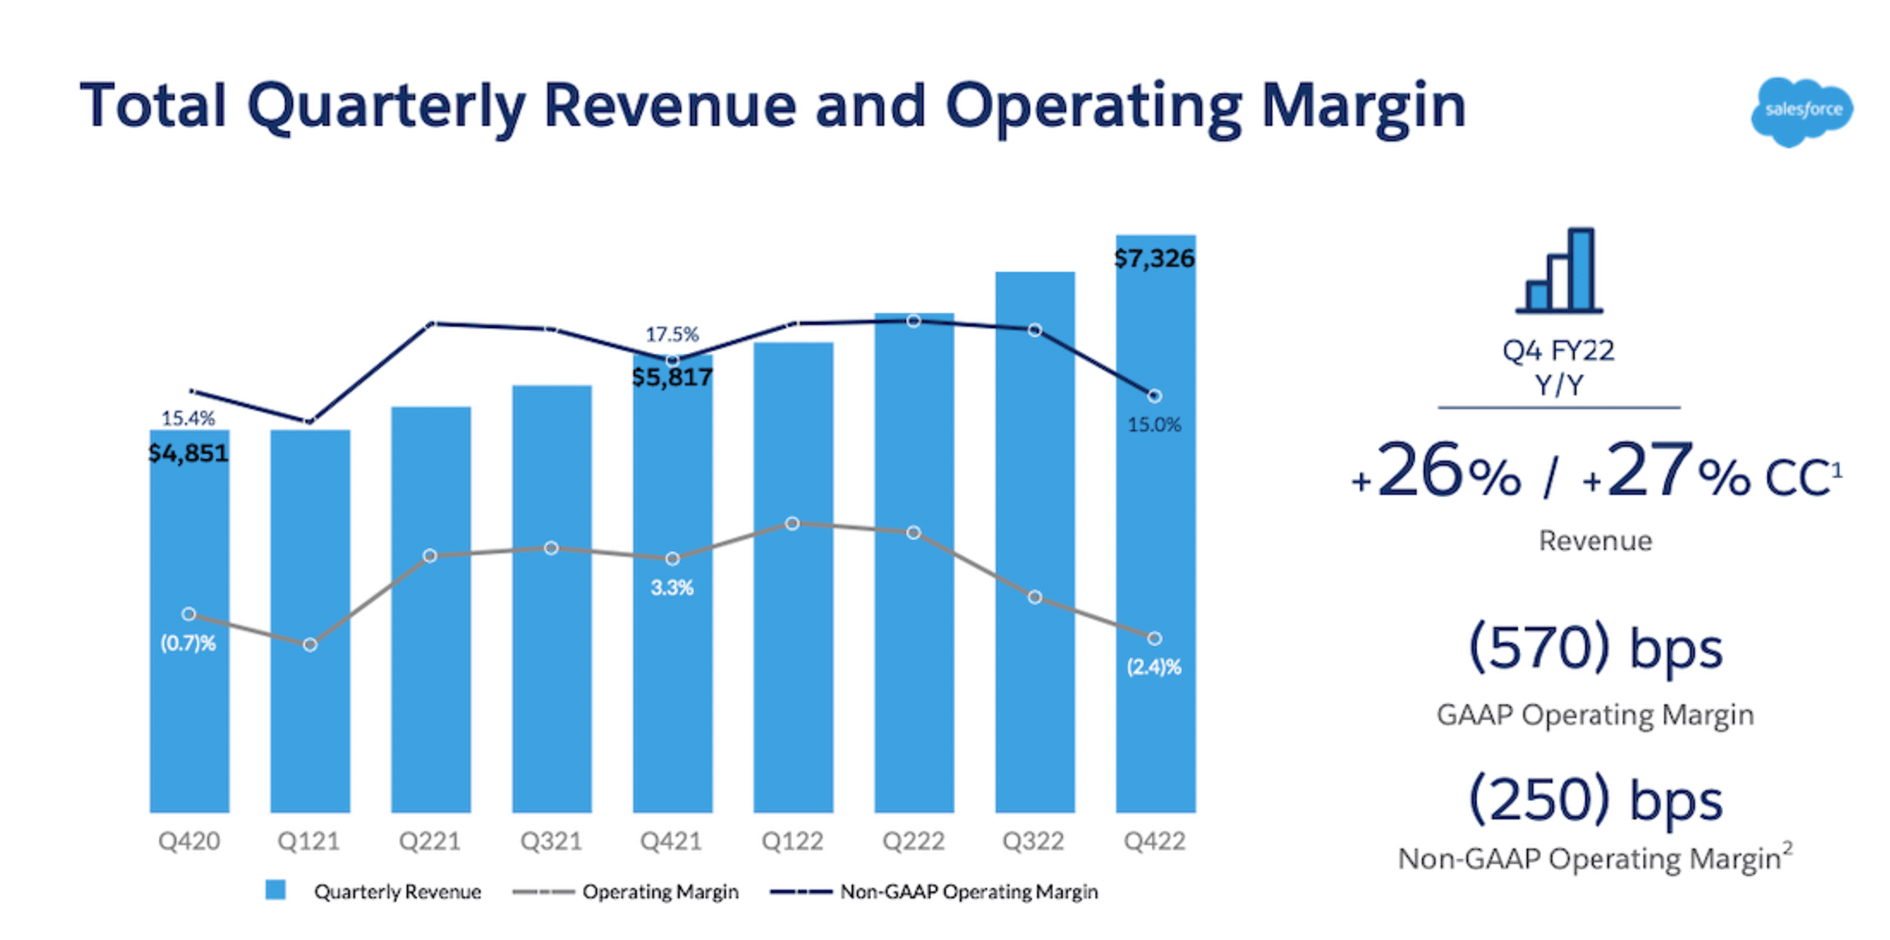
\includegraphics[width=0.8\textwidth]{Chapter1_Introduction/Pictures/Saleforce_Quaterly_Revenue.png}}
    \caption{SAP S/4HANA and Salesforce Market Share and Revenue Growth}
    \label{fig:salesforce_revenue}
\end{figure}


\subsection{Cost Efficiency and Performance Gains}
Organizations that have adopted SAP S/4HANA report substantial cost savings and operational improvements:
\begin{itemize}
    \item Fjellsport reduced inventory costs by 20\% through SAP S/4HANA’s real-time analytics \cite{sap_2025}.
    \item ENEL improved its billing efficiency by 50\%, enhancing cash flow management \cite{sap_2025}.
    \item Swiss Port Ltd lowered its TCO by 30\%, demonstrating the cost-effectiveness of SAP S/4HANA \cite{sap_2025}.
\end{itemize}

Similarly, Salesforce remains a high-ROI investment, with its Service Cloud alone generating \$8 billion in 2024, proving its financial sustainability and continued market growth \cite{statista_2023b}.


\subsection{Justification for This Research}

SAP S/4HANA is the largest and most dominant ERP system in the enterprise software market, trusted by the majority of Fortune 500 companies. Although SAP provides its own CRM solutions, adding SAP CRM to an existing SAP S/4HANA landscape represents a significant financial investment, making it impractical for many organizations. However, SAP's third-party CRM integration capabilities allow businesses to connect best-in-class solutions without committing to an entirely SAP-exclusive ecosystem.

Similarly, Salesforce stands as the largest CRM provider in the world, offering unparalleled CRM features. Salesforce natively supports third-party ERP integrations via APIs, allowing seamless DS between customer-facing processes and back-end ERP.

From a financial and operational standpoint, integrating SAP S/4HANA with Salesforce provides the best of both worlds leveraging SAP’s industry-leading ERP capabilities while taking advantage of Salesforce’s best-in-class CRM features. This integration ensures:
\begin{itemize}
    \item Cost-effectiveness, avoiding the high investment required for SAP's native CRM.
    \item Seamless interoperability, utilizing SAP’s support for third-party CRM solutions and Salesforce’s API-driven ERP integration.
    \item Optimized enterprise efficiency, combining the world’s most powerful ERP and CRM into a unified system.
\end{itemize}

Given that SAP is the undisputed leader in ERP solutions and Salesforce holds the largest market share in CRM, it makes both strategic and financial sense for businesses to integrate these two dominant systems. By doing so, organizations can maximize efficiency, reduce costs, and achieve seamless business operations without compromising on functionality.

This research will focus on how businesses can optimally integrate SAP S/4HANA and Salesforce, ensuring data consistency, automated workflows, and future proof system scalability. The findings will serve as a guide for companies looking to leverage this integration for financial and operational success.



%%%%%%%%%%%%%%%%%%%% Conclusion
\section{Conclusion}

The literature review in this thesis serves as the foundation for understanding the integration of SAP S/4HANA and Salesforce using SAP BTP Integration Suite. As enterprises increasingly rely on ERP and CRM systems to drive operational efficiency, the demand for seamless integration between these platforms has become paramount. However, achieving this integration is not without challenges, as evident from the extensive body of research analyzed in this chapter.

A key takeaway from the literature is the evolution of ERP and CRM systems. Initially, ERP was developed to centralize business processes, while CRM emerged as a specialized tool for managing customer interactions. Over the years, these systems have become indispensable, yet they largely function in silos. While SAP S/4HANA provides robust ERP capabilities, its CRM functionalities are limited compared to specialized platforms like Salesforce. This necessitates integration to ensure real-time DS, operational efficiency, and an enhanced customer experience.

One of the most pressing challenges in ERP-CRM integration is DS and consistency. Multiple studies indicate that data fragmentation occurs when ERP and CRM systems store information in separate databases, leading to discrepancies in customer records, order details, and sales forecasts. This fragmentation is exacerbated by differences in data structures, formats, and identifiers used in SAP S/4HANA and Salesforce. The literature highlights the need for middleware solutions to act as a bridge, ensuring seamless communication between these systems.

The second major challenge discussed is technical barriers, particularly API mismatches, security concerns, and performance limitations. SAP S/4HANA primarily relies on OData and SOAP-based web services, whereas Salesforce uses RESTful APIs and GraphQL, creating interoperability issues. Additionally, security concerns such as data protection, authentication, and encryption present obstacles to effective integration. Research has shown that enterprises must carefully design their integration architecture to balance security with real-time data access.

Given these challenges, middleware solutions have gained prominence as a viable approach to ERP-CRM integration. SAP BTP (BTP) Integration Suite has been identified as a leading middleware option, offering pre-built iFlows, API management, and monitoring tools. Unlike third-party solutions such as MuleSoft and Dell Boomi, SAP BTP provides native integration capabilities tailored for SAP environments. Its low-code/no-code interface, combined with pre-configured connectors for Salesforce, makes it an ideal choice for businesses leveraging both platforms.

A key contribution of this chapter is the assessment of SAP BTP's role in ERP-CRM integration. Studies indicate that SAP BTP excels in data transformation, real-time analytics, and compliance management. By providing built-in connectors for Salesforce and SAP S/4HANA, it reduces the complexity associated with custom integration efforts. Furthermore, its support for hybrid and multi-cloud architectures ensures flexibility for organizations operating in diverse IT landscapes.

Despite its advantages, SAP BTP is not without limitations. The literature review highlights research gaps, particularly the lack of practical implementation studies. While many studies discuss ERP-CRM integration in a theoretical or strategic context, few provide detailed technical guidance on configuring SAP BTP for SAP-Salesforce integration. This gap underscores the need for an implementation-focused study, which this thesis aims to address.

Another research gap identified is the lack of comparative analyses between SAP BTP and other middleware solutions specifically in the context of SAP S/4HANA and Salesforce integration. While this thesis does not focus on middleware comparisons, it acknowledges the potential benefits of evaluating how different middleware platforms handle data orchestration, security, and performance optimization.

Future trends in ERP-CRM integration, as explored in this chapter, suggest that AI-driven data mapping, serverless integration, and regulatory compliance will play an increasingly critical role. AI and ML can automate data transformation, reduce mapping errors, and optimize synchronization processes. Additionally, the rise of serverless middleware solutions presents new opportunities for scalable and cost-effective integrations.

From a compliance perspective, organizations must ensure GDPR, SOX, and industry-specific regulatory adherence when integrating ERP and CRM systems. The literature emphasizes that data protection mechanisms, audit trails, and access controls are crucial to preventing security breaches and maintaining trust in integrated environments.

The insights gathered from this literature review inform the direction of this thesis. Given the lack of practical implementation research, this study aims to provide a structured guide on integrating SAP S/4HANA and Salesforce using SAP BTP Integration Suite. By detailing the architecture, data mappings, API configurations, and real-world testing, this research will contribute a hands-on approach to middleware-based ERP-CRM integration.

Furthermore, this literature review lays the groundwork for the next chapter, which focuses on defining the business problem and case analysis. While this chapter provided a theoretical foundation, the next chapter will translate these insights into real-world business challenges, use cases, and justifications for implementing SAP BTP as the middleware of choice.

In conclusion, this literature review underscores the critical need for seamless ERP-CRM integration, the challenges associated with achieving it, and the role of middleware—specifically SAP BTP—in bridging the gap between SAP S/4HANA and Salesforce. While existing research highlights various strategies and potential solutions, it lacks a practical implementation guide, which this thesis seeks to provide. The findings of this chapter set the stage for a technical deep dive into SAP BTP’s capabilities and its application in a real-world business context.

%=== END OF CHAPTER TWO ===
\newpage


